\chapter{Background}
\label{ch:background}

% material necessary to understand the rest of the thesis

% last section in this chapter is usually related work

\com{
\todo[inline]{When you do your literature study, you should have a nearly complete Chapters 1 and 2.\\
You may also find it convenient to introduce the future work section into your report early – so that you can put things that you think about but decide not to do now into this section.\\
Note that later you can move things between this future work section and what you have done as you may change your mind about what to do now versus what to put off to future work.
}

What does a reader (another x student -- where x is your study line) need to know to understand your report?
What have others already done? (This is the “related work”.) Explain what and
how prior work / prior research will be applied on or used in the degree
project /work (described in this thesis). Explain why and what is not used in
the degree project and give valid reasons for rejecting the work/research.
}


\noindent This chapter presents relevant research background needed to understand the current state of the art of localisation and mapping.
Firstly, the coordinate frames of the wheeled mobile robot are presented to define how the robotic lawn mower will be localised, controlled, and constrained.
Afterwards, the focus will be on localisation, starting from an analysis of sensors available on \glspl{ALM} and other useful for positioning in outdoor settings.
The focus is on sensors which require no additional infrastructure installation.
Additionally, sensor fusion techniques to exploit their measurements will be presented to later explain which technique is the most relevant for this project.
Furthermore, a brief analysis of mapping aspects is presented.
Different algorithms are available, but only the most relevant approach is discussed.
Finally, theoretical related works are briefly described to highlight their contributions regarding this thesis, and a summary of the lessons learned from the literature study is presented.


\section{Wheeled Mobile Robots}

\noindent Mobile robots are able to move themselves in the environment they are in.
The one used in this thesis equips two standard back wheels with differential drive and two castor wheels on the front, which allow free rotation around the wheel axle for multiple direction steering.
An analysis of the coordinate and robot frame is presented, followed by the definition of its kinematic model and related constraint.

\subsection{Coordinate Frame}

\noindent
The \gls{2D} pose of the robot, ${pose}$, in the global frame $G$ is defined by the following vector:
\begin{equation}
    pose = \begin{bmatrix}x_{pose}&y_{pose}&\theta_{pose}\end{bmatrix}^T
    \label{eq:dof}
\end{equation} where the coordinates $x_r$ and $y_r$ define the position of $O_R$ in $O_G$, and $\theta_r$ defines the relative rotation angle between the $X_R$ direction axis of the robot and the related global axis $X_G$, as shown in figure \ref{fig:TikzKine}.
\begin{figure}[!ht]
    \centering
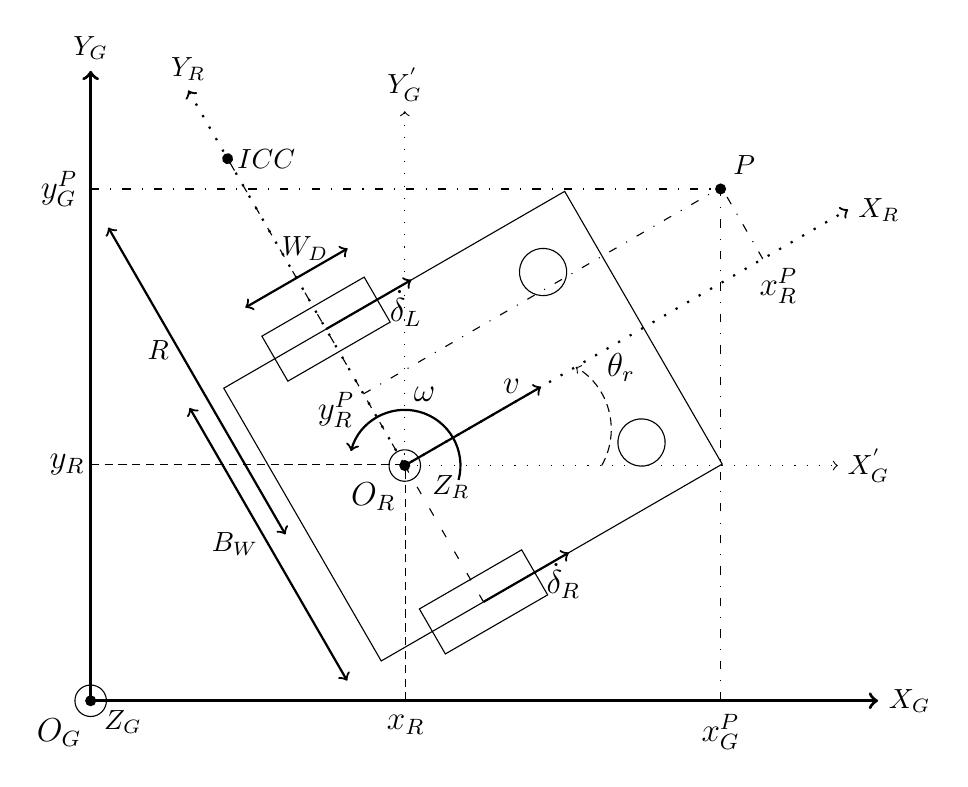
\begin{tikzpicture}
  \draw [<->, very thick]  (0,8) node (yaxis) [above] {$Y_G$} |- (10,0) node (xaxis) [right] {$X_G$};
  \draw (-0.4,-0.4)  node (origin) [] {\large$O_G$};
  \draw (4,-0.3)  node (x_r) [] {\large$x_R$};
  \draw (-0.3,3)  node (y_r) [] {\large$y_R$};
  
  \draw (8,-0.4)  node (x_i) [] {\large$x_G^P$};
  \draw (-0.4,6.5)  node (y_i) [] {\large$y_G^P$};
  \draw (8.3,6.8)  node (p) [] {$P$};
  \fill[black]  (8,6.5)   circle (2pt);
  \draw[ loosely dashdotted] (8,0) -- (8,6.5);
  \draw[ loosely dashdotted] (0,6.5) -- (8,6.5);
  
  \draw[black] (0, 0) circle (0.2) node (z) [below] {~~$~~~~~Z_G$};
  \fill[black]  (0,0)   circle (2pt);
  \draw[ densely dashed] (4,0) -- (4,3);
  \draw[ densely dashed] (0,3) -- (4,3);
  \begin{scope}[xshift=113.5, yshift=85]
        \fill[black]  (0,0)   circle (2pt);
          \draw [<->, loosely dotted]  (0,4.5) node (yaxisG) [above] {$Y_G^{'}$} |- (5.5,0) node (xaxisG) [right] {$X_G^{'}$};
          \draw (-0.4,-0.4)  node (origin_r) [] {\large$O_R$};
          \draw[->, densely dashed]  (2.5,0) to[out=60,in=-30, distance=0.5cm] (2.17,1.25) node (theta) [below, right] {\large$~~\theta_r$} ;
      \begin{scope}[rotate=30]
          \draw [<->, loosely dotted, thick]  (0,5.5) node (yaxis_r) [above] {$Y_R$}
                |- (6.5,0) node (xaxis_r) [right] {$X_R$};
          \draw[->, thick]  (0.5,-0.5) to[out=45,in=-45] (0.5,0.5)  node (omega) [above] {\large$~\omega$} to[out=135,in=45] (-0.5,0.5);
          \draw [->, thick] (0,0) -- (2,0) node (vel) [above, left] {\large$v$~~};
          \draw [->, thick] (0,2) -- (1.25,2) node (v_L) [below] {\large$\dot \delta _L$~~};
          \draw [->, thick] (0,-2) -- (1.25,-2) node (v_R) [below] {\large$\dot \delta _R$~~};
          \draw[<->, thick]  (-2,-2) -- (-2,2) node (base) [pos=0.5, below, left] {$~B_W$} ;
          \draw[<->, thick]  (-0.75,2.75) -- (0.75,2.75) node (diameter) [above, left] {$W_D$~~} ;
          \draw[<->, thick]  (-1.75,0) -- (-1.75,4.5) node (curvature) [pos=0.6, below, left] {$R$} ;
          \draw[-, loosely dashed]  (0,-2) -- (0,4.5) ;
            \fill[black]  (0,4.5)   circle (2pt);
            \draw (0,4.5)  node (ICC) [above, right] {$ICC$};
        \draw[black]  (-0.75,-2.33) rectangle (0.75,-1.67);
        \draw[black]  (-0.75,2.33) rectangle (0.75,1.67);
        \draw[black] (-1.5,-2) rectangle (3.5,2);
        \draw[black] (2.75, 1.25) circle (0.3);
        \draw[black] (2.75, -1.25) circle (0.3);
        \draw[black] (0, 0) circle (0.2) node (z) [below] {~~$~~~~~~~~Z_R$};
        
        
          \draw (5.25,-0.4)  node (x_i) [] {\large$x_R^P$};
          \draw (-0.4,1.05)  node (y_i) [] {\large$y_R^P$};
          \draw[ loosely dashdotted] (5.25,0) -- (5.25,1.05);
          \draw[ loosely dashdotted] (0,1.05) -- (5.25,1.05);
      \end{scope}
  \end{scope}
\end{tikzpicture}
  \caption{Kinematic model of a differential drive mobile robot.}
  \label{fig:TikzKine}
\end{figure}

The translational and rotational relations from a robot frame point $P_R=[x_R^P,y_R^P,1]^T$ to its global corresponding $P_G=[x_R^G,y_R^G,1]^T$ are defined by the transformation matrix $T^G_R$.
\begin{align}
P_{G} = T^G_R \cdot P_{R} && \text{with } && T^G_R =
\begin{bmatrix}
\cos(\theta_r) & -\sin(\theta_r) & x_R \\
\sin(\theta_r) & \cos(\theta_r) & y_R \\
0 & 0 & 1 \\
\end{bmatrix}
\label{eq:transfPoint}
\end{align}
Every roto-translation of points in the \gls{2D} plane is uniquely defined by the equations~\ref{eq:transfPoint}.  
Other transformation matrices are not relevant for the case study.


\subsection{Kinematic Analysis}
\label{ssec:kin_a}
\noindent
For the scope of this thesis, the kinematics are considered. Other aspects, such as torque, friction, physical implications, and in general the dynamics of the systems, are not relevant to be analysed for the scope of this thesis.

The direct kinematic equations are defined as follows.
The \gls{ALM} consists of two drive back wheels mounted along the same axis.
Each wheel is actuated independently either in forward or backward rotation.
By individually setting the velocity of each wheel, the robot rotates around a different \gls{ICC}~\cite{ICC}, $ICC$ in figure \ref{fig:TikzKine}.
This point is defined in the $Y_R$ axis by its distance, $R$, from the robot's origin:
\begin{equation}
    R = \cfrac{\dot \delta_R + \dot \delta_L}{\dot \delta_R - \dot \delta_L} \cdot \cfrac{B_W}{2}
    \label{eq:R}
\end{equation}
where $\dot \delta_R$, $\dot \delta_L$ are the perceived velocities of the right and left wheel respectively, and $B_W$ defines the base width of the \gls{ALM} as distance between the wheels.
Using this approach it is possible to vary the trajectory that the robot follows by varying the wheels' velocities.
In case the wheels' velocities are equal, $R$ will result to be infinite and the robot will not rotate, following a straight trajectory.
%Some constraints about the possible trajectories are explained in section \ref{sec:constraints}.
The rate of rotation about $ICC$ is the same as the angular velocity around the robot frame's origin $O_R$, defined by the time derivation of its orientation $\theta_r$. 
This angular velocity, $\omega$, is used to control the trajectory of the robot and its derivative is defined as:
\begin{equation}
    \omega = \cfrac{\partial{\theta_r}}{\partial{t}} = \cfrac{\dot \delta_R - \dot \delta_L}{B_W}
    \label{eq:omega}
\end{equation}
where $\partial{t}$ is the partial timestamp used to derive the velocity from the partial angle displacement $\partial{\theta_r}$.

The \gls{ALM} is controlled through the desired linear velocity $v$ along the $X_R$ axis of the robot, and the desired angular velocity $\omega$ around the $Z_R$ axis.
The angular velocity is defined above in equation \eqref{eq:omega} and the linear velocity can be defined as a transformation of either the angular velocity or the wheels' velocities, as in:
\begin{equation}
    v = \omega \cdot R = \cfrac{\dot \delta_R + \dot \delta_L}{2}
    \label{eq:vel}
\end{equation}

The inverse kinematics are defined as follows.
The \gls{ALM} model is controlled by differential drive kinematics as it is propelled by two separate motors mounted on the back wheels, and its movements are defined by the wheel actuators. The desired control velocities need to be transformed into the wheels' velocities using:
\begin{align}
    \dot \delta _L  & = v - \omega \cdot \frac{B_W}{2} & , &&
    \dot \delta _R  & = v + \omega \cdot \frac{B_W}{2} \quad .
    \label{eq:wheel_vel}
\end{align}


\subsection{Constraints}
\label{sec:constraints}
\noindent
This differential drive system is not able to move immediately in every direction along the \gls{2D} environment.
The degrees of freedom, defined in \eqref{eq:dof}, are fewer than degrees of mobility, given by the control velocities, $v$ and $\omega$.
The system is thus called non-holonomic and at least a non-holonomic constraint has to be defined for it.
A non-holonomic rolling constraint could be set for the standard wheels used by the differential mobile robot, as the wheels spin purely along their orientation.
For example, to allow the robot to perform a rolling motion along the $Y_R$ axis, the robot will have to vary the velocity of each wheel to rotate around its origin, aligning itself along that desired direction, before moving forward.

Non-holonomic constraints do not allow for the integration of the differential equations to retrieve the final pose, since the displacements of each wheel are not sufficient to determine it.
This implies that the position and orientation need to be estimated using the integration of wheels' velocities, rather than their position displacements.
An integrable approach can be used to estimate its pose with a sufficient sampling rate, but the usage of incremental displacements provided by integration of wheels' velocity measurements will inevitably accumulate errors over time, causing a drift on the pose estimates.

\com{
\section{Localisation}
\noindent As this is the main topic of this project, an extensive analysis of this field will be performed.
Understanding the current state-of-the-art of localisation and its possible improvement is required.

Firstly, the available sensors that could be installed directly on the mobile robot, that do not require additional installation of infrastructures, and that can be used to improve localisation are described below.

Afterwards, different techniques available to fuse their heterogeneous measurements are described in their performances.
}

\section{Sensors}
\noindent For a robot to localise itself, it needs to perceive its surroundings using measurements of its sensors, which perceive and interpret different phenomena based on their characteristics.
They can be classifies into two main different types~\cite{perception}.
\textit{Proprioceptive sensors} measure values internal to the robot's system, while it interacts with the environment. They provide a value of how the movements of the mobile robot are perceived with respect to the outside, e.g., wheel encoders, accelerometers, or gyroscopes.
\textit{Exteroceptive sensors} provide measurements related directly to their perception of the robot's environment. The information they measure are related to phenomena happening at the environments around the mobile robot, e.g., magnetometers, \glspl{GNSS}, or cameras.
As they measure different aspects, their capabilities differ based on the phenomenon they measure and on the .
They provide different sampling rates and measured states, which need to be combined to exploit their characteristics and limit their inaccuracies.

An overview is presented below to introduce the available sensors installed on the \gls{ALM} and adopted to improve localisation.

\subsection{Wheel Encoder}

\noindent This proprioceptive sensor detects the number of revolutions of the wheels, and they can be used to estimate their velocity~\cite{encoder}. An example of an optical wheel encoder is given in Figure \ref{fig:encoder}.
\begin{figure}[!ht]
  \begin{center}
    \includegraphics[width=0.65\textwidth]{Images/2-Background/Enc.jpg}
  \end{center}
  \caption{Optical wheel encoder and resulting encoded signal~\cite{wheelEncoder}.}
  \label{fig:encoder}
\end{figure}

This sensor relies on a rotary encoding disk attached to the wheel axis on the end of the motor that estimates the relative angle change of the wheel.
Rotary encoders can be of different kinds based on which phenomenon they observe: mechanical, optical, or magnetic.
Incremental encoders estimate the relative rotation of the wheels by detecting the number of pulses, defined by the step signals A and B in Figure \ref{fig:encoder}, within certain time period using the internal clock of the embedded computer.

Wheel encoders are often chosen for the estimation of the pose, as their measurements can be used through integration with the previous estimate of the robot's pose to provide the next pose estimate.
This process is called \gls{DR} and the pose estimate provided is called \gls{WO}.
Related to the field of sensor fusion, since they provide measurements with an high sampling rate and they are inexpensive, their employment is common to compute a short-term accurate \gls{DR}.
However, it is subjects to errors and their accumulation, given that only velocity measurements are used.
Some non-systematic errors related to these sensors are the miscalculations caused by slippage, uneven terrain, and other environmental issues which include wheels' temperature and the pressure of their tires.
In order to improve its \gls{DR} estimates, other sensors' measurements need to be combined with its velocity estimates to get rid of the integration drift error accumulation on its position calculations.


\subsection{Inertial Measurement Unit}

\noindent An \gls{IMU} is an inertial sensor which is used to detect multiple phenomena and whose measurements are relative to the inertial frame of the platform they are attached to.
They perceive both proprioceptive elements through accelerometers and gyroscopes, and exteroceptive characteristics through magnetometers.
Recent \glspl{IMU} are developed on \glspl{MEMS} which are inexpensive and provide measurements with high sampling rates.
These sensors are placed in each orthogonal axis to provide measurements for each degree of freedom in free space, as shown in Figure \ref{fig:imu}.
\begin{figure}[!ht]
  \begin{center}
    \includegraphics[width=0.5\textwidth]{Images/2-Background/IMU-2021-04-23 14-13-19.png}
  \end{center}
  \caption{Structure of accelerometers and gyroscopes of an \Gls{IMU}~\cite{inertial}.}
  \label{fig:imu}
\end{figure}

Accelerometers measure linear acceleration, gyroscopes output the perceived angular velocity, and magnetometers provide measurements about the surrounding magnetic field.
Knowing these quantities, the position and orientation can be estimated by integrating those signals over time with a \gls{DR} approach~\cite{indr}.
Their measurement are prone both to deterministic errors, such as repeatable terms and temperature induced variations, and to stochastic errors, such as switch-on to switch-on variations and in-run variations~\cite{magnusson_improving_2012}.
Deterministic errors can be compensated for through prediction and calibration, while stochastic ones are more difficult to model because of their noise and randomness.

Accelerometers and Gyroscopes, as they measure proprioceptive characteristics, are sensors that provide measurements which are not conditioned by external conditions or disturbances.
Magnetometers, instead, might be conditioned by external disturbances as the magnetic field can be affected by multiple external factors, as any electronic device has a magnetic influence.

They provide accurate results over a short time span, but the integration of noisy measurements implies an accumulation of these errors over time. This phenomenon then leads to a diverging drift effect, if not corrected by other sensor measurements.


\subsection{Global Navigation Satellite System}

\noindent \glspl{GNSS} are exteroceptive systems based on signals received from satellites orbiting earth.
A \gls{GNSS} receiver uses trilateration to estimate its position on the globe using the time of flight of the signals sent by specific satellites.  %, used to calibrate the \gls{3D} pose and time difference. 
The messages sent by them include their trajectories and their internal reference timestamp. 
As soon as the position and time difference are known, those are used to estimate the pose of the robot using pseudo-ranges, as shown in Figure \ref{fig:gps}.
\begin{figure}[!ht]
  \begin{center}
    \includegraphics[width=0.5\textwidth]{Images/2-Background/KaiBorre-p73.png}
  \end{center}
  \caption{\Gls{GNSS} trilateration from known position of four satellites~\cite{Borre2007}.}
  \label{fig:gps}
\end{figure}

The spatial configuration of the satellites determines the localisation accuracy. 
Close position of several satellites implies that their range will be close, and the messages they provide will not be as useful for trilateration.
A more spread configuration of satellites' range reduces the \gls{DOP}, which compares the position error to the satellite range error.
Other source for error is related to the positioning in dense and noisy environments, due to multi-path effects of the signals.
The performance of these sensors is thus highly dependent on their environment.

For the \gls{GNSS} receiver to estimate its position, it need to acquire measurements from at least four satellites~\cite{Borre2007}.
The four satellites signals are used both to trilaterate the \gls{3D} position and to synchronise of the clocks, essential to compensate eventual time differences between the receiver and the satellites.
In case the perceived satellites are fewer than four, the receiver will have a system outage, not being able to estimate its position and velocity.
As now there exists multiple \gls{GNSS} constellations developed by distinct space agencies, the latest \gls{GNSS} sensors are able to receive signals from multiple satellite systems to improve their satellite coverage and their precision.
With a higher number of perceived satellite signals, the receiver is able to use redundant information to increase its robustness to external disturbances and improve its position measurement accuracy.

The sampling rate of \gls{GNSS} receivers is usually \SI{1}{Hz}, thus, used alone it is too slow for real-time applications of positioning for vehicles. 
However, it offers global measurements, which are not subject to drift errors and therefore they can be used to correct \gls{DR} estimates.


\subsection{Camera}

\noindent A camera sensor is an exteroceptive sensors, usually composed of lenses and light sensors, which gathers the \gls{RGB} information from the environment.
Recent camera models, e.g., structured-light cameras, are also able to estimate depth measurements. %estimate stereopsis data, used
They project an infrared mesh pattern in the environment and then use stereo cameras to perceive this pattern, trilaterating the depth distance based on the density of the projected points.
Multiple factors can lower this sensor's performances, such as excessive lightning conditions and reflecting materials which modify the infrared pattern.

These sensors provide \gls{VO} estimating the incremental movement of the camera by detecting changes in adjacent images with a \gls{F2F} method~\cite{camera}~\cite{cameraa}.
The \gls{VO} algorithm identifies the position of some specific features and then matches those landmarks in consecutive images.
Knowing their relative pose changes it is possible to estimate the corresponding camera movement.
The performance relies on the identification of landmarks, the more visible and variant landmarks are identified, the more the pose estimation will be accurate as the landmarks' difference will be more prominent.
%Those features can be computed using different descriptors, e.g. \gls{SIFT}, \gls{SURF}, or \gls{ORB}.
The matching phase is guided by an initial estimate of the camera movement which projects previously found features to search just along that projection.
The landmarks are matched after passing a consistency test and those displacements are triangulated to estimate the camera pose through a bundle adjustment step~\cite{robustFusion}, as shown in Figure \ref{fig:camera}.

\begin{figure}[!ht]
  \begin{center}
    \includegraphics[width=0.65\textwidth]{Images/2-Background/VO.pdf}
  \end{center}
  \caption{Motion estimation via \gls{F2F} methodology~\cite{camera}~\cite{cameraa}.}
  \label{fig:camera}
\end{figure}

Instead of using a more complex \gls{SLAM} algorithm, where all the position of the landmarks are also used to estimate a map of the environment, with the \gls{VO} approach the landmarks are only used for displacement analysis, without storing the landmark positions over time.
Using this technique, only the previous state will be saved to estimate the position offset, resulting in faster computations and thus higher sampling frame rates.
This is a key aspect, since the aim is to use this approach inside an embedded system for a real-time application. 
However, the measurements provided from the \gls{VO} are estimates in velocity between frames and they need to be integrated to compute a \gls{DR} localisation, which is subject to drift.

%Different techniques are available to compute the features and derive the estimations from the frames, with different implementations such as ORB-SLAM2 and RTABMap, where each of them provide odometry measure with different settings. Some examples are briefly shown in~\cite{Fast and robust visual odometry with a low-cost IMU in dynamic environments Erliang Yao, Hexin Zhang and Haitao Song}

Given its exteroceptive characteristics, the \gls{VO} has a low frequency sampling rate.
Therefore, the \gls{VO} estimations will result to be inaccurate while going at high velocity as it makes the landmarks identification too complex for the \gls{F2F} algorithm.



\section{Sensor Fusion}

\noindent
In the field of localisation for mobile robots, sensor fusion is employed to combine redundant and complementary measurements from heterogeneous sensors to gain a more precise understanding of the pose in the environment.
An issue related to the sensor fusion problem is the determination of the best configuration to combine the measurements of multiple different sensors.
The objective of sensor fusion is to merge the knowledge acquired by these sensors to improve the position estimate with a more accurate solution with respect to any of the individual data sources, trying to mitigate their drawbacks and to maintain their best provided features~\cite{mitchell_multi-sensor_2007}.

Sensor fusion could be characterised based on \textit{competitive}, \textit{complementary}, and \textit{cooperative} approaches~\cite{1199023}.
\textit{Competitive} fusion is defined when the same states of a system are estimated by different sensors, before being fused to increase the system's robustness.
In \textit{complementary} fusion, the observations of different phenomena, which are different but connected through kinematics or dynamics aspects, are merged to describe the complete system's state.
\textit{Cooperative} fusion focused on combining raw measurements from different sensors to provide information that will not be obtained by a single source.
In ~\cite{weckenmann_multisensor_2009}, the \textit{time domain} is also considered to classify sensor fusion techniques which manage measurements arriving at different times to increase the reliability the evolution of the estimates.

%Sensor fusion is related to independent measurements and it can be classified into multiple categories: \textit{sensors}, \textit{states}, \textit{domains}, and \textit{time}
%The fusion across different sensors involves merging the same measured phenomenon from different devices to increase the robustness of the measured data, in a \textit{competitive} approach.
%Fusion among different states is focused on sensors which estimate , improving their precision in a \textit{complementary} way.
%Different domains are fused when sensors measure the same attribute with a different range or frame, improving their performances when one of these sensors reaches its limits, through a \textit{cooperative} procedure.

The most common approach to sensor fusion is through the usage of statistical methods, where the uncertainties of the sensors are described by probabilistic models~\cite{gustafsson_statistical_2010}.
This section will describe the basics of some statistical filters used for sensor fusion purposes.
The \gls{KF} will be detailed as it is the most basic among them, followed by an analysis of its non-linear correspondent, the \gls{EKF}. 

\subsection{Kalman Filter}

\noindent The \gls{KF} was first developed by R.E. Kalman in~\cite{kalman} as a Bayesian estimator used in linear Gaussian systems.
It can recover information about the state of a signal, even when it is disturbed by noise or incomplete, and it is is often used for real-time, embedded, and sensor fusion systems.
Starting from a linear dynamic system model, governed by the following equations:
\begin{align}
 \label{eq:dyn-mod-s}
    \mathbf{X}_{t+1} & = A \cdot \mathbf{X}_t + B \cdot \mathbf{u}_t  + C \cdot \mathbf{q}_t \\
 \label{eq:dyn-mod-m}
    \mathbf{Z}_{t+1} & = H \cdot \mathbf{X}_t \qquad \quad ~~ + \mathbf{r}_t 
\end{align}
with its Gaussian noises described by $\mathbf{q}_t \sim \mathcal{N}\left(0, Q\right)$ and $\mathbf{r}_t \sim \mathcal{N}\left(0, R\right)$, the \gls{KF} estimates the states using a feedback-control loop of prediction and correction steps.

It uses a recursive probabilistic approach to efficiently filter discrete estimates of the states of a process and its estimated uncertainty.
Then, it corrects its state and decreases its uncertainty using new measurements with the goal of minimising the \gls{LMSE}.
To reach an optimal estimation, at each iteration it performs a weighted sum of its current estimate using both the prior estimate and the new measurements, weighting them based on their relative uncertainty.
The \gls{KF} holds information about its estimate and uncertainty respectively through the state vector $\mathbf{X}_t$, which contains the states and descriptions of the system, and the state covariance matrix $P_t$,  which holds information about the variance between those states as statistical error indicator.
It is structured as continuous cycle of its iterative process and it does not require to store in memory the history of the previous states and they are computationally efficient.

The prediction phase estimates the next state based on the previous one and eventual control inputs.%, and adding Gaussian white noise to account for uncertainties in the prediction estimate.
\com{
We proceed under the Markovian assumption that p(xk)=∫∞−∞p(xk|xk−1)p(xk−1)dxk−1, meaning that the distribution over the state of an object at time k can be predicted entirely from its state at previous time k−1. (\url{https://stonesoup.readthedocs.io/en/latest/auto_tutorials/01_KalmanFilterTutorial.html#prediction})
}
First of all, the \gls{KF} computes the prediction of the current state $\hat{\mathbf{X}}_{t+1}^-$ assuming its previous estimate as  $\text{E}[\mathbf{X}_{t}] = \mathbf{X}_{t}^-$ , using the transition matrix $A$ and eventual inputs $B \cdot \mathbf{u}_t$, as derived in the following:%, and the state noise vector $\boldsymbol \eta_t$:%, as in equation \eqref{eq:pred-state}:
\begin{align}
\begin{split}
\hat{\mathbf{X}}_{t+1}^- & = \text{E}[\mathbf{X}_{t+1}] = \text{E}[ A \cdot \mathbf{X}_t + B \cdot \mathbf{u}_t + C \cdot  \mathbf{q}_t] \\
& =  A \cdot \text{E}[\mathbf{X}_t] + B \cdot \mathbf{u}_t + 0 \\
& =  A \cdot \mathbf{X}_t^- + B \cdot \mathbf{u}_t
  \label{eq:pred-state}
\end{split}
\end{align}
%where %$\hat{\mathbf{X}}_{t+1}$ is the state of the system%, being a Gaussian random variable, can be described with its mean and covariance as $\mathbf{X}_{t} \sim \mathcal{N}\left(\mathbf{X}_{t},P_{t}\right)$, its Gaussian noise is described by $\boldsymbol \eta_t \sim \mathcal{N}\left(0, Q\right)$.
Then, the prediction of the current state covariance $\hat{P}_{t+1}$ is computed using the previous state covariance $P_t$, the transition matrix $A$, and the state noise covariance $Q$:%, as in equation \eqref{eq:pred-cov-p}.
    \begin{align}
\begin{split}
    	\label{eq:pred-cov-p}
        \hat{P}_{t+1} & = \text{Cov}[\mathbf{X}_{t+1}] = \text{Cov}[A \cdot \mathbf{X}_t] + \text{Cov}[B \cdot \mathbf{u}_t] + \text{Cov}[C \cdot \mathbf{q}_t] \\ & = A \cdot P_t \cdot A^T + C \cdot Q \cdot C^T % Kind of wrong as we miss B*G*B^T
\end{split}
    \end{align}


After noisy measurements $\mathbf{Z}_{t+1}$ have been obtained, the correction phase corrects the prediction based on the uncertainty of both the prediction and the measurements to improve the estimation of the state.
As the initial step in the correction, the prediction of the estimated measurements, $\hat{\mathbf{Z}}_{t+1}$, is obtained using the measurements matrix $H$:
    \begin{align}
    \hat{\mathbf{Z}}_{t+1} & = H \cdot \hat{\mathbf{X}}_{t+1}^-
    \label{eq:pred-measure}
    \end{align}
Then, the innovation vector, $\mathbf{Y}_{t+1}$, is computed as the difference between the estimated measurements and the actual measurements $\mathbf{Z}_{t+1}$:
    \begin{align}
    \mathbf{Y}_{t+1} & = \mathbf{Z}_{t+1} - \hat{\mathbf{Z}}_{t+1}
    \end{align}
Its related innovation covariance, $S$, is given by the following formula, where $R$ is the measurements' process noise:
    \begin{align}
    S & = H \cdot \hat{P}_{t+1} \cdot H^T + R
    \end{align}
The Kalman gain, $K$, is then computed to improve the state estimate as a relation between state covariance and innovation covariance, as follows:
    \begin{align}
    K & = \hat{P}_{t+1} \cdot H^T \cdot S^{-1}
    \end{align}
The corrected estimate, $\mathbf{X}_{t+1}^-$, is finally obtained using the predicted estimate and the innovation vector weighted by the innovation covariance, as:% in equation \eqref{eq:correct-state}.
    \begin{align}
    \mathbf{X}_{t+1}^- & = \hat{\mathbf{X}}_{t+1}^- + K \cdot \mathbf{Y}_{t+1}
    \label{eq:correct-state}
    \end{align}
Finally, the corrected covariance matrix of the state, $P_{t+1}$, is:% obtained by equation \eqref{eq:standard-corr-cov}.
    \begin{align}
    	\label{eq:standard-corr-cov}
    P_{t+1} & = (I - K \cdot H) \cdot \hat{P}_{t+1}
    \end{align}

After this, the loop of equations restarts from the prediction phase by updating the time index from $t+1$ to $t$, following the structure defined in Figure \ref{pic:kalm}.

\tikzstyle{block} = [draw, rectangle, minimum width=6em, align=center,fill=gray!5]
\tikzstyle{arrow} = [-latex, very thick]
\newcommand*{\tran}{\top}

\begin{figure}[!ht]
\centering
\begin{tikzpicture}[auto, node distance=2cm,>=latex']
    \setlength{\abovedisplayskip}{0pt}

    % Place the blocks
    \node[text width=1cm, rounded corners=3pt, block,
          label={[above,align=center]{Initial State}}] at (-2, 0) (initial)
          {\begin{align*}\mathbf{X}_0^- \\ P_0\end{align*}};
    \node at (0.0, 0.0) (sum) {};
    \node[block, text width=6cm,
          label={[above,align=center]{Prediction}}] at (4, 0) (prediction)
          {\begin{align*}
        \hat{\mathbf{X}}_{t+1}^- & = A \cdot \mathbf{X}_t^- + B \cdot \mathbf{u}_t \\ % + \boldsymbol \eta_t\\
        \hat{P}_{t+1} & = A \cdot P_t \cdot A^T +  C \cdot Q \cdot C^T
           \end{align*}};
    \node [block, right of=prediction,
            node distance=3cm, text width=2.4cm,
            label=above right:{New}, label=below right:{Measure}] at (5, -1.33) (iterUpdate)
            {$\mathbf{Z}_{t+1}$};
    \node [block, left of=prediction,
            node distance=3cm, text width=2.4cm,
            label=left:{Next step}] at (2.8, -1.33) (iterChange)
            {$$t+1 \rightarrow t $$ };
    \node [block, text width=6cm,
           label={[above,align=center]{Correction}}] at (4, -4) (innovation)
           {\begin{align*}
    \hat{\mathbf{Z}}_{t+1} & = H \cdot \hat{\mathbf{X}}_{t+1}^-\\
    \mathbf{Y}_{t+1} & = \mathbf{Z}_{t+1} - \hat{\mathbf{Z}}_{t+1}\\
    S & = H \cdot \hat{P}_{t+1} \cdot H^T + R\\
    K & = \hat{P}_{t+1} \cdot H^T \cdot S^{-1} \\
    \mathbf{X}_{t+1}^- & = \hat{\mathbf{X}}_{t+1}^- + K \cdot \mathbf{Y}_{t+1}\\
    P_{t+1} & = (I - K \cdot H) \cdot \hat{P}_{t+1}
            \end{align*}};

    % Connect the nodes
    \draw [arrow] (initial) -- (prediction);
    \draw [arrow] (prediction.east) -| (iterUpdate.north);
    \draw [arrow] (iterUpdate) |- (innovation);
    \draw [arrow] (innovation.west) -|  (iterChange);
    \draw [arrow] (iterChange) |-  (prediction);

\end{tikzpicture}

  \caption{Structure of the Kalman Filter}
  \label{pic:kalm}
\end{figure}

Its many components can are structured in multiple ways, based on the problem and model specification.
The initial state $\mathbf{X}_{0}^-$ can be defined either by zeros or by starting estimates according to the first measurements.
The starting uncertainty of the filter $P_0$ can be initialized directly with the state noise covariance in case of unavailability of good initial values. In both cases, the filter will need some steps before converging to more stable estimates of state and covariance.
The state noise covariance $Q$ is harder to determine and it is usually tuned to training data.
The measurement noise covariance $R$ is composed by the variances of its measurements' components and they are usually estimated through calibration or sensors' data sheets.
If the state and measurement noises change over time, their matrices $Q$ and $R$ needs to be updated as the filter runs, as it is their relative ratio which determines how the Kalman gain $K$ is defined to improve the estimates. In this case, the \gls{KF} can be defined as Adaptive~\cite{adaptive}~\cite{1099422}.


An numerical evaluation improvement over the standard \gls{KF} is directly given by changing the state covariance correction step using the Joseph’s form~\cite{schmidt_analysis_2010}.% defined by equation \eqref{eq:joseph}:
\begin{equation}
    P_{t+1} = (I - K \cdot H) \cdot \hat{P}_{t+1} \cdot (I - K \cdot H)^T + K \cdot R \cdot K^T
    \label{eq:joseph}
\end{equation}
As the standard state covariance correction in Equation \eqref{eq:standard-corr-cov} is composed by a subtraction and a multiplication, it can result in a loss in symmetry and positive-definiteness due to rounding errors in a finite word length computer.
The Joseph’s form state covariance correction instead maintains positive and non-zero eigenvalues in $P_t$ through the addition of two positive semi-definite matrices, given that $\hat{P}_{t+1}$ and $R$ are positive semi-definite as well, which is valid up to numerical precision.
The additional stability of the covariance propagation is obtained with this more computationally demanding equation~\cite{BarShalom2001EstimationWA}.

The filter is considered an optimal estimator in a mean square sense only if the disturbances in both the process and measurements can be modelled as Gaussian white noise.
Moreover, the prediction and correction phases are formulated with the assumptions that the state $\mathbf{X}_t^-$ is markovian, i.e., that is evolution depends solely on its previous value, and that the measurement $\mathbf{Z}_{t+1}$ only depends on the state $\mathbf{X}_{t+1}^-$, and not on previous measurements.
When these assumptions hold, the \gls{KF} is the optimal linear estimator.
However, it can be used with reasonable results even if the assumptions do not hold, i.e., when the noise is not Gaussian and the system is non-linear, but in those cases other filters will perform better and should be preferred, such as the ones described below and in Appendix \ref{ch:non-linear}.
In any case, as the \gls{KF} needs multiple iterations to stabilise and the performance of the algorithm should not account for the first steps.

\subsection{Extended Kalman Filter}

\noindent The \gls{EKF} is an extension of the \gls{KF} used to estimate non-linear systems, where the dynamic system model equations \eqref{eq:dyn-mod-s} and \eqref{eq:dyn-mod-m} are generalised, respectively, as follows:
\begin{align}
\label{eq:nonlinearf}
&\mathbf{X}_{t+1}  =  f_1(\mathbf{X}_{t}, \mathbf{u}_t)& + ~~~~   f_2(\mathbf{q}_t) &&
    \textrm{where}~\mathbf{q}_t \sim \mathcal{N}(0, Q)\\
&\mathbf{Z}_{t+1}  =  g_1(\mathbf{X}_{t+1}) & + ~~~~ g_2(\mathbf{r}_t) &&
    \textrm{where}~\mathbf{r}_t \sim \mathcal{N}(0, R)
\end{align}
where $f_1$ and $g_1$ are the non-linear transformation and measurement functions, respectively.


The problem related to non-linear system is given by the fact that, although the initial states are Gaussian random variables, their related propagation might not be Gaussian anymore as they are obtained through non-linear transformations. The difference with respect to linear systems is that linear transformations of Gaussian random variables remain random variables.
Therefore, these non-linear outputs could not be used to propagate the estimates and the covariances using the \gls{KF} equations.

The \gls{EKF} propagates the states using the non-linear functions and the covariances through a linearisation of them around the previous states' estimates, exploiting the Taylor's expansion~\cite{thrun_probabilistic_2005}.
The Jacobian matrices obtained are used as approximation for the linear transformation of the system~\cite{1386886}:
\newcommand{\partialat}[2]{\frac{\partial {#1}}{\partial {#2}}}
\begin{align}
F = \partialat{f_1}{\mathbf{X}_{t}}\Bigr|_{\mathbf{X}_{t} = \mathbf{X}_{t}^-} & &
G = \partialat{g_1}{\hat{\mathbf{X}}_{t+1}}\Bigr|_{\mathbf{X}_{t+1} = \mathbf{X}_{t+1}^-}
\end{align}
where $F$ is the approximation of the transition matrix $A$, and $G$ is the approximation of the measurement matrix $H$, as defined in the linear equations \eqref{eq:dyn-mod-s} and \eqref{eq:dyn-mod-m}.
As the linear approximation of the \gls{EKF} is based on the first-order derivatives, it provides only first-order accuracy of covariance. In case of highly non-linear systems, this procedure can inject errors in the system and cause divergence of the filtered estimate.

\section{Mapping}

\noindent For a mobile robot to navigate in an area, it is essential to understand its position in a map that represents its environment.
There exists two main types of maps: \textit{topological maps} which describes the connectivity
of identified features in the environment as nodes in a graph connected by paths as edges, and \textit{metric maps} which employs a coordinate system to describe the properties of the environment.
Moreover, maps can also be defined based on their perspective: \textit{world-centric} maps where a global coordinate space is used and every object has a global coordinate, and \textit{robot-centric} maps where each point is defined with respect to the robot's pose and measurements.

%\subsection{Occupancy Grid}
A widely used kind of maps is the Occupancy grid.
It projects a \gls{3D} environment into a \gls{2D} abstraction and it is commonly used to aid the localisation features of mobile robots.
Occupancy grids are world-centric metric maps which are composed of occupancy probabilities cells.
Their representation of the environment is defined by evenly spaced cells, each one represents a random variable which describes the uncertainty of the presence of an obstacle within its coordinates~\cite{thrun_probabilistic_2005}.
While the mobile robot moves in that map, the measurements obtained can be used to update the probability of nearby cells using approximate posterior estimates.



\section{Related Works}

\noindent
%It has emerged thanks to a set of research outcomes which have provided tools to increase the possible features that a \gls{ALM} can achieve.
The improvement of an \gls{ALM} is a research topic which has motivated the research and development of multiple projects, which will be presented below.
They provide a complete analysis of all the components and a comprehensive view about the improved features, e.g., localisation and mapping, to be provided on such a robotic lawn mower.
The complete development of a fully featured mobile robot for golf course mowing, as part of a yearly robotics course, is detailed in~\cite{noauthor_groundsbot_nodate}.
A recent master thesis about the development of robotic lawn mower with Visual SLAM and terrain classifier is described in~\cite{lukas_robotic_2020}.
A bachelor thesis regarding the prototyping of a mower using a camera and GPS in available in~ \cite{andersson_smart_2018}.
%Both of these works did not manage to deliver the desired objectives of being fully autonomous, considering the construction of the mower's infrastructure and given their time constraints.

Different approaches for localisation on a \gls{HRP} have been developed: using \gls{GPSRTK} external infrastructure~\cite{oden_localization_2017}, and using \gls{UWB} sensors on the mower~\cite{lensund_local_2018}.
In these cases, however, there is a requirement for external devices to localise the \gls{ALM} and this aspect is not part of the scope of this thesis.


A review about techniques for localisation and mapping for autonomous systems is provided in~\cite{9065135}, where the focus is about the definition of sensors' performance and the description of different map features.

Extensive analyses of the techniques used by autonomous robots that have to deal with real-world sensor data and mapping using their measurements are provided in~\cite{thrun_probabilistic_2005},~\cite{gustafsson_statistical_2010} and~\cite{mitchell2007multi}, which are well-cited references for estimation tasks.

\subsection{State-of-the-art Localisation}
\noindent An implementation of a \gls{EKF} described in~\cite{moore_generalized_2016} provides a introduction for the development of a localisation module, including the modularity requirement for the configuration of different sensors.
%A discussion about the improvements and limitations offered by each sensor is included, along with a comprehensive description of their implementation, which allows for the fusion of measurements from multiple and heterogeneous sensors.% in the \gls{ROS} framework.
%Their \texttt{robot\_localization} ROS package\footnote{\url{http://wiki.ros.org/robot_localization}}  implements multiple nodes to provide an easy way to fuse data from multiple and heterogeneous sensors.
However, the final performance and static configuration do not allow for the implementation of a real-time adaptive system which needs updates with an high frequency.

Other approaches to sensor fusion using the \gls{KF} to merge the measures of the available sensors are described in the literature.
In~\cite{801027}, an analysis about the difference of performance between \glspl{KF} driven by the kinematic model or by the \gls{WO} measurements is described. 
As a conclusion, while their performance are similar, the kinematic driven prediction phase \gls{KF} are preferred.


Some references which use an \gls{EKF} to merge measurements from a similar set of sensors available on a different mobile robot than the one discussed in this thesis are described below.
In~\cite{9024731} an \gls{EKF} is used to merge the \gls{WO} and \gls{VO} with \gls{GNSS} and \gls{IMU} measures.
Multiple \glspl{EKF} are employed in series in~\cite{9075286} to merge the \gls{WO} and \gls{VO} with \gls{GNSS} and \gls{IMU} measures.
An adaptive approach using the \texttt{robot\_localization} package to merge \gls{WO}, \gls{GNSS} measures, \gls{IMU} measures, and \gls{VO} is defined in~\cite{CHEN1298238}.
In~\cite{magnusson_improving_2012}, an \gls{EKF} is adopted to improve the localisation of a vehicle using \gls{WO}, one \gls{GNSS} receiver, and one \gls{IMU}.
In~\cite{8c506f630d4e478dace903637fa0a75b}, an approach to deal with delayed measurements in the \gls{EKF} is presented to fuse \gls{WO}, one \gls{GNSS} receiver, and one \gls{IMU}.
In~\cite{king_low_2008} and~\cite{skog2005low}, an \gls{EKF} is adopted to provide localisation for a mobile robot using inexpensive sensors, such as \gls{GNSS} receiver and \gls{IMU}.

The adaptive \gls{KF} has been in use for a while and some references are described below.
An adaptive approach for the generation of noise covariances in the \gls{KF} to account for dynamic noise in sensor fusion to improve \gls{GPS} estimation with inertial measures from a \gls{IMU} is defined in~\cite{mohamed1999adaptive}.
In~\cite{grandoni_sensor_2001}, the adaptive approach is applied to an \gls{EKF}.
In~\cite{kong_using_2012},~\cite{Werries-2016-5519}, and~\cite{hao_modified_2018}, adaptive approaches using \gls{EKF} are adopted to merge measurements obtained respectively by one \gls{GNSS} receiver, by one \gls{GNSS} receiver and one \gls{IMU}, and by two \gls{GNSS} receivers and one \gls{IMU}.
In~\cite{chenavier_position_1992}, an adaptive approach to sensor fusion using \gls{EKF} is used to merge measurements from \gls{WO} and \gls{VO}.
%In~\cite{li_high-precision_2013}, a Multi-State-Constraint \gls{EKF} is adopted to fuse the measurement obtained by visual odometry and one \gls{IMU}.


Comparisons about different configurations of sensor fusion approaches are defined in the following references.
In~\cite{amador_robot_2019}, a comparison about the fusion of \gls{WO}, \gls{GNSS}, and \gls{IMU} using \gls{EKF} and \gls{UKF}, described in \ref{sec:ukf}, is presented. It highlights how the \gls{EKF} provides more accurate and faster results than the \gls{UKF}.
In~\cite{7373480}, an \gls{EKF} is adopted to improve the localisation of a mobile robot using different configurations with a wheel encoder, a magnetic compass, one \gls{GNSS} receiver, and one \gls{IMU}. The most accurate results have been obtained by the approach fusing all their measures.
In~\cite{8696103}, different configurations of sensors including \gls{WO}, \gls{GNSS} receiver and \gls{IMU} are fused with an \gls{EKF} and analysed. The most accurate results have been obtained fusing all sensors' measurements.
Multiple \glspl{KF} are used in~\cite{liu2016stereo} to merge \gls{VO} and \gls{IMU}, and to discuss the related improvements provided by different configurations.
To improve the non-linearity performances, an implementation of the \gls{IEKF} with a \gls{IMU} and \gls{VO} system is described in~\cite{bloesch2017iterated}.


\subsection{State-of-the-art Mapping} 
\noindent The mapping feature has been discussed in the literature using multiple techniques.
As the focus of this thesis is related to the usage of occupancy grids, their presence in the state-of-the-art implementation is analysed.

In \cite{joubert2012adaptive}, an algorithm based on the Bayes Theorem is provided to update the cells of an occupancy grid considering measurements from a sensor which estimates its distance to its surroundings.
It is specified that it has been derived and improved from~\cite{thrun_probabilistic_2005} and~\cite{12145}.
A similar approach has been presented in \cite{singh_sonar_2019}, where the sensor of choice to detect the environment is the sonar sensor.
In these two approaches, two separate occupancy grids managed by different algorithms are used to describe the emptiness and occupancy aspects of the environment. 
A final process is then performed to merge their knowledge, using the most probable cells to update the map and allowing to have a more reliable final result.

Using these occupancy grids and probabilities to define the map of the mobile robot, negative values could be used to define the virtual boundaries~\cite{thrun_probabilistic_2005}.
By initialising the map with a random uncertainty, the mobile robot will be able to move freely inside its boundaries and as soon as it approximates to an negative cell, it will change its direction to avoid getting out of its limits.
At the same time, it will be able to use its sensors to perceive its surroundings and update the occupancy cells based on the identified obstacles within it.

%Finally, once a better certainty about its knowledge of the map in reached, the mobile robot could employ path planning algorithms to improve its coverage performance.
%An algorithm based on Occupancy Grids for terrain mapping using sensor information is available at~\cite{Saranya2016OccupancyGB}.


\section{Summary}
\com{
It is nice to have this chapter conclude with a summary. For example,you can include a table that summarizes other people’s ideas and benefits and drawbacks with each - so as later you can compare your solution to each of them. This will also help you define the variables that you will use for your evaluation.
}

\noindent The key lessons learned during this background analysis and description can be summarised by the following points.
\begin{itemize}
    \item A localisation module could be built starting from a mobile robot and its kinematic analysis. Additionally, sensors could be added with a modular approach to provide measurements improving the positioning performance.% and the usage of that \gls{ROS}-enabled mobile platform to easily test and compare the results of different configurations of sensors;
    \item The sensors available are enough to provide both the position and velocity measurements needed to improve the localisation aspects of a mobile robot, without requiring a lawn infrastructure installed;
    \item Statistical sensor fusion techniques enable for the merging of measurements from different and heterogeneous sensors with performances which are robust and fast enough to be implemented in an embedded device;
    The \gls{EKF} provides good estimates and it can be tuned updating the noises which characterise the system according to sensor's measures, as the localisation scope requires.
    \item Occupancy grids provide a \gls{2D} abstractions of the environment which can account both for the definitions of its boundaries and for the presence of obstacles within it.
    \item The usage of collision events to update the knowledge of the cells in the occupancy grid is possible using bayesan's posterior estimates.
    %\item numerous related studies and implementations have been developed in similar topics to improve localisation and mapping features.%, and the analysis of an optimal configuration of sensors which require no external installations is still relevant to the best of the found knowledge.
\end{itemize}



\cleardoublepage
%\clearpage
